\documentclass[12pt]{report}
\usepackage{graphicx}
\usepackage{booktabs}
\graphicspath{ {images/} }
\usepackage[english]{babel}
\usepackage{graphicx}
\begin{document}
\title{Lab6 \\ Specific Heat of Solids Revisited \\ Physics 132}
\author{Dominic Martinez-Ta}
\date{22 May 2015}
\maketitle


\section{Purpose}
	
	The purpose of this experiment is to test three different well known models of specific heat capacitance over 
the temeprature range of approximately 200k to 350k  for two different solid materials(Chromium and Copper[Cu]).
 We will measure the $C_v(T)$ of two different solids by preparing a series of temperature baths, and fit $C_v(T)$
 to the three models below, and analyze the results.

\begin{equation}
Dulong-Petit: c_v = 3R = 3N_Ak_b
\end{equation}

\begin{equation}
Einstein-Solid: c_v = 3R\frac{(\frac{T_E}{T})^2e^{\frac{T_E}{T}}}{(e^{\frac{T_E}{T}}-1)^2}
\end{equation}

\begin{equation}
Debye-Model: c_v = \frac{12\pi^4}{5}R\frac{T^3}{T_D^3}
\end{equation}

Where the gas constant is $R = 8.314 J\cdot K^{-1}\cdot  Mol^{-1}$

\section {Materials and resources}

Data Studio, Water, Salt, Hot water, Dry Ice, Thermometers, Pressure meter, copper, chromium, Love.

\section{Procedure}

	Create a series of hot and cold temperature baths to measure the specific heat of two solids. 
This lab will be divided into two parts, so it is highly recommended to complete Part I for both samples first, and complete
 Part II for both samples last.\\
\\
\textbf{Part I: Use hot and cold water for:}
	\[ 5^{\circ}C < T < 80^{\circ}C\]
\textbf{Part II: Use ethanol and dry ice for}
	\[-70^{\circ}C<T<5^{\circ}C\]
\textbf{Collect at least} 10 $C_v(T)$ data points for each sample, approximately 5 $C_v(T)$ data points or more
in each Part. The data points should be spaced by approximately $15^{\circ}C$ To do this, keep $T_H \sim T_C+15^{\circ}C$
 so that the cold baths have the following temperatures (or similar temperatures):
\[T_c(^{\circ}C) = 65, 50, 35,20,5,0,-10,-25,-40,-55,-70\]
\begin{itemize}
	\item Increase precision (significant figures) of temperature sensor to highest accuracy when collecting data
	\item If the cold water bath temperature does not change significantly, consider:
	\begin{itemize}
		\item Decreasing amount of water in cold bath
		\item Increasing difference between $T_H$ and $T_C$
	\end{itemize}
	\item It is possible to increase the experimental accuracy by repeating measurements and taking the average value, 
which may be considered if time permits
\end{itemize}


\section{Data Analysis}
	 From our Data in \textbf{Part I} it appears that our mass and change in temperature appears to have changed in a 
somewhat linear fashion until we reached the very low temperatures. (Below $0^{\circ}C$). However, when measuring the weight, we had an error of $\pm 0.07$, skewing our accuracy for the weight of the samples. \\
	\\When measuring the temperature, we had an error from outside heat sources. This is because our thermometer was exposed to not only the liquid we were dipping it in, but at the same time was exposed to air. This would have resulted in our temperature readings being off by about $\pm 2^{\circ}C$. This is because the temperature of the air could have been significantly higher than our liquid. And thus forcing us to having to wait a while until our systema and the thermometer to reach equilibrium. \\
	\\From \textbf{Part II} of our experiment, we saw that we had lost mass at constant rates when we used the Ethanol Alcohol and the dry ice. For the most part, this part of the experiment went well except for when we transferred our sample from the warmer bath to the colder bath. We could have, and most likely have, lost some heat due to the temperature of the air outside of the baths. For that, we can safely assume that the error of the sample temperature would be $\pm 2^{\circ}C$. \\
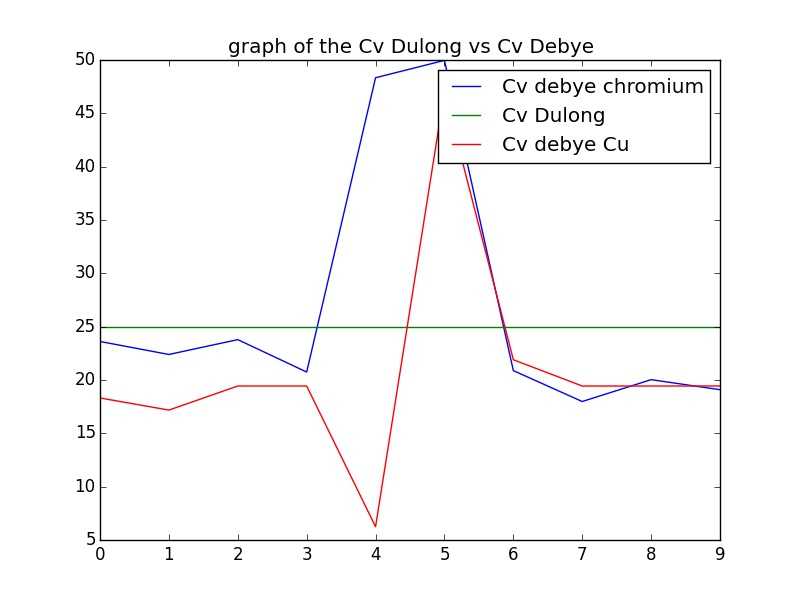
\includegraphics[scale=0.5]{chromium_debye&cudebye}\\
Graph of the Chromium and Cu Debye model for $C_v$ compared to the Dulong-Petit model.\\
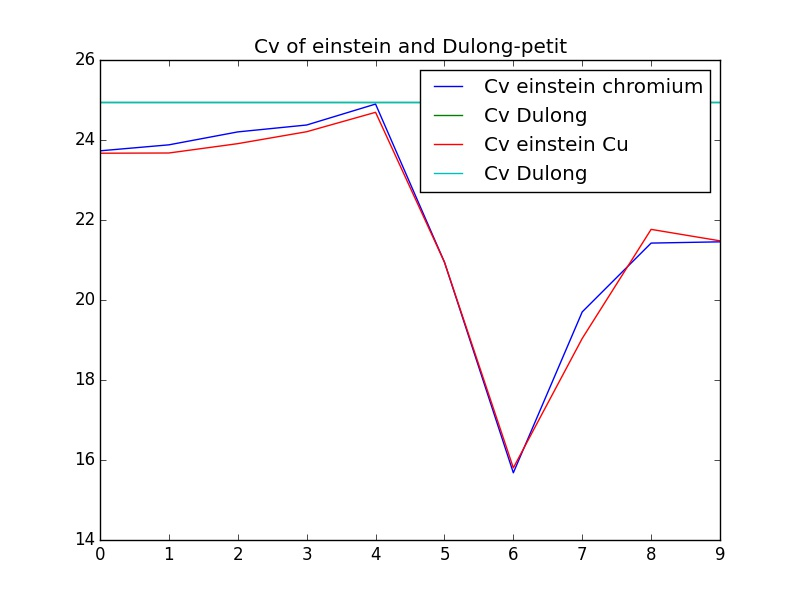
\includegraphics[scale=0.5]{chromium_einstein}\\
Graph of the $C_v$ of Chromium and Cu for the Einstein solid compared to the Dulong-Petit Model.
\section{Questions}
	\begin{enumerate}
		\item Scientific measurements involve error, including systematic, resolution and
			random error. Comment on the systematic errors present when obtaining
			heat $Q_{sample}$, and identify as many forms of systematic error as possible.
		\item How can this experiment be improved? Consider how it may be improved
			without much effort (i.e. low budget), and how it may be improved while
			affording a large budget for laboratory equipment (i.e. using expensive
			equipment such as highly accurate temperature probes).
		\item The Dulong and Petit model predicts $c_v = 3R = 24.9 J\cdot mol^{-1} \cdot K^{-1}$ for all solids,
			however, experimentally solids have been shown to have different heat
			capacities from this value. Why does this occur?
		\item How did Debye’s model for specific heat improve upon the Einstein Solid?
		\item At extremely low temperatures, even the Debye model has been shown to
			break down. Why does this occur?
	\end{enumerate}
\section{Answers to questions}
	\begin{enumerate}
		\item Discussed in \textbf{Data Analysis}
		\item This experiment can be improved by using a larger bath for our temperatures. This is because the larger 				the bath, our error caused by the temperature of the air would have been around 0. This is because the 			air temperature would be around the temperature of the baths.  This is for if we had a low budget. 					However, if we had a large budget and were being funded in a laboratory environment. We would be 				able to actually create the equipment necessary to cool our baths to certain temperatures with almost 				perfect accuracy.  
		\item This occurs because we have different formations in the structures of our objects. Some parts of our 				objects may have a certain element that the other does not which effects the way energy is 						transferred. Gold for example has a high heat capacity, while regular plastic does not. Why is that?					That's because of the structure of object and the amout of energy it takes to excite these atoms. Each 				atom is different (if they aren't of the same element) and that means that different energies is needed           to change the phase-state of the object.
		\item "Thus, the second model to test is the Einstein Solid model, which quantizes lattice vibrations as phonons and assumes an ensemble of N quantum harmonic oscillators, each oscillator with three degrees of freedom, so
that all 3N normal modes of oscillation have frequency $v_E$. Above some temperature $T_E$, where
$T_E = \frac{hν_Ε}{k_B}$, Einstein’s model returns its value to the high temperature limit of Dulong and Petit."
This was basically explained in question 3. A summary of what was said is that we have degrees of freedoms to take into account now, thanks for the improvement by the Einstein Solid. 
		\item This occurs because at extremely low temperatures, it will take very little energy needed to excit our atoms and to cause heat to be transferred. Therefore, it's extremely easy to transfer heat at low temperatures thus showing that extremely low temperatures, the Debye Model breaks down. 
	\end{enumerate}
\section{Conclusion}
	We can conclude that our experiment was a success due to the small amount of errors that we had measured. We thus proved that solids have different heat capacities and how these heat capacities are affected at extremely low temperatures. At moderate temperatures, we saw that these heat capacities remain at a near constant. Showing to us how heat  is lose when it is transferred from different objects.
\section{Data}

\begin{center}

\begin{table}[h]
\textbf{Part I}, chromium \\
 $\begin{array}{ *{7}{c} }
\toprule
T_H(C) & T_C(C) & T_F(C) & M_{Total}(g) &  m_{H_2O}(g) & m_{cup}(g) & m_{chromium}(g) \\
\midrule
77.0 & 63.7 & 59.7 & 145.73 & 136.22 & 2.00 & 7.51 \\ 
65.7 & 49.9 & 47.6 & 125.88 & 115.37 & - & -\\ 
52.5 & 33.8 & 31.6 & 125.76 & 116.25 & - & - \\ 
34.6 & 18.6 & 18.2 & 126.42 & 116.91 & - & - \\ 
21.4 & 4.2 & 3.1 & 122.34 & 112.83 & - & - \\ 
\end{array}$
\end{table}
\end{center}
\begin{center}
\begin{table}[h]
\textbf{Part I}, Copper \\
 $\begin{array}{ *{7}{c} }
\toprule
T_H(C) & T_C(C) & T_F(C) & M_{Total}(g) &  m_{H_2O}(g) & m_{cup}(g) & m_{Cu}(g) \\
\midrule
77.0 & 60.0 & 61.2 & 142.00 & 100.00 & 2.00 & 40.00 \\ 
65.7 & 50.0 & 52.1 &  148.00 & 106.00 & - & - \\ 
48.6 &  34.7 & 34.7 & 153.30 & 113.30 & - & - \\ 
35.0 &  21.0 &  21.0 &  134.43 &  92.43 & - & - \\ 
21.0 & 5.0 &  7.3 &  95.7 & 53.7 & - & - \\ 
 \end{array}$
\end{table}
\begin{table}[h]
\textbf{Part II}, Chromium \\
 $\begin{array}{ *{9}{c} }
\toprule
T_H(C) & T_C(C) & T_F(C) & M_{Total}(g) &  m_{eth}(g) & m_{cup}(g) & m_{chromium}(g)  & \frac{\partial m}{\partial t} & \Delta t(s)\\
5.0 & -10.0 & -7.3 & 40.2 & 10.0 & 2.0 &  7.51 & 0.02 & 7 \\
-10.11 & -25 & -24.41 & 38.5 & - & - & - & 0.01 & 8 \\
-24.12 & -40.0 & -41.05 & 40.5 & - & - & - & 0.03 & 3 \\
-40.00 & -55.0 & -54.45 & 44.6 & - & - & - & 0.02 & 5 \\
-55.7 &  -75.0& -74.45 & 38.2 & - & - & - & 0.08 & 13 \\
\midrule
\end{array}$
\end{table}
\begin{table}[h]
\textbf{Part II}, Copper \\
 $\begin{array}{ *{9}{c} }
\toprule
T_H(C) & T_C(C) & T_F(C) & M_{Total}(g) &  m_{eth}(g) & m_{cup}(g) & m_{Cu}(g)  & \frac{\partial m}{\partial t} & \Delta t(s)\\
5.0 & -9.8 & -7.3 & 40.2 & 10.0 & 2.0 &  40.0 & 0.13 & 10 \\
-10.2 & -25.4 & -24.41 & 38.5 & - & - & - & 0.15 & 9 \\
-22.5 & -39.9 & -41.05 & 40.5 & - & - & - & 0.09 & 9 \\
-42.3 & -56.2 & -54.45 & 44.6 & - & - & - & 0.15 & 11 \\
-55.2 &  -75.5 & -74.48 & 38.2 & - & - & - & 0.07 & 13 \\
\midrule
\end{array}$
\end{table}
\end{center}
\end{document}